\documentclass[11pt]{article}
\usepackage[margin=1in]{geometry}
\usepackage{amsmath,amssymb,amsthm,mathtools}
\usepackage{booktabs,graphicx,siunitx,microtype,url}
\usepackage[colorlinks=true,allcolors=blue!55!black]{hyperref}
\usepackage[numbers,sort&compress]{natbib}

\sisetup{scientific-notation=true, round-mode=figures, round-precision=2}

\newtheorem{theorem}{Theorem}
\newtheorem{proposition}[theorem]{Proposition}
\newtheorem{lemma}[theorem]{Lemma}
\newtheorem{corollary}[theorem]{Corollary}
\theoremstyle{definition}
\newtheorem{definition}[theorem]{Definition}
\newtheorem{remark}[theorem]{Remark}

\DeclareMathOperator{\SO}{SO}
\DeclareMathOperator{\Ortho}{O}
\DeclareMathOperator{\Hom}{Hom}
\DeclareMathOperator{\End}{End}
\DeclareMathOperator{\Sym}{Sym}
\DeclareMathOperator{\rank}{rank}
\DeclareMathOperator{\tr}{tr}
\DeclareMathOperator{\range}{range}
\newcommand{\R}{\mathbb{R}}
\newcommand{\Vdip}{V_{\mathrm{dip}}}
\newcommand{\Vres}{V_{\mathrm{res}}}
\newcommand{\Veight}{V_{8}}
\newcommand{\rhoext}{\rho}

\title{\bfseries Equivariant Representation Learning for a Physically Known,\\
Non-Orthogonal Group: the Case of the 12-Lead Electrocardiogram}
\author{}
\date{}

\begin{document}
\maketitle

\begin{abstract}
Equivariant deep learning almost always begins by \emph{assuming} a symmetry --- image
rotations, permutations of a set --- and almost always assumes that the group acts
\emph{orthogonally}, because that is what makes the steerable-kernel machinery work.
We study a setting in which the symmetry is instead \emph{derived from physics}, is
exactly computable, is clinically interpretable, and is \emph{not orthogonal}. Under
the equivalent cardiac-dipole model the 12-lead electrocardiogram (ECG) is a fixed
linear image $x = Dv$ of a three-dimensional heart vector $v$, and changes of posture,
respiration and electrode placement act as $v \mapsto Rv$ with $R \in \SO(3)$. The
induced action on lead space, $x \mapsto DRD^{+}x$, is a faithful three-parameter Lie
group action that is \emph{not} orthogonal in the Euclidean geometry of lead space:
for the standard Dower transform the anisotropy is $\kappa(D) = 1.45$ and for the Kors
transform $2.19$.

We give (i) a complete characterisation of the equivariant linear maps for this
action, via an explicit gauge in which it becomes the standard representation of
$\SO(3)$, verified numerically against the Schur-lemma prediction; (ii) a sharpened
account of where the existing generalisation theory for equivariant models actually
breaks under a non-orthogonal action --- not in $L^2(\mu)$, where it survives
untouched, but in the \emph{estimator's} geometry, where the Reynolds operator becomes
an oblique projection --- together with the repair and its exact constant; (iii)
identifiability conditions for the decomposition of a representation into invariant
(pathology) and equivariant (pose) parts, with the three strata of the condition made
explicit; and (iv) a diagnostic that measures how much of a pretrained ECG encoder's
capacity is spent modelling the nuisance orbit.

Empirically, our gauge-equivariant network is invariant to floating-point precision
($\num{7e-7}$ relative), whereas a network built on the usual orthogonality assumption
errs by $\num{4e-2}$ and a conventional CNN by $0.99$. The sample-efficiency picture is
more nuanced than the folklore: the constraint is a clear win in the small-data
regime and a measurable \emph{cost} once labels are plentiful, and we locate the
crossover. We report this rather than tuning it away, and give the accompanying
approximate-equivariance and pose-aware variants that recover the deficit.
\end{abstract}

\section{Introduction}

The design of equivariant architectures is now a mature craft, but it rests on an
assumption that is rarely examined because it is usually true by construction: that
the group acts on the input space by \emph{orthogonal} (more generally unitary)
transformations. Steerable CNNs, tensor-field networks, spherical CNNs and their
descendants \citep{cohen2016gcnn,cohen2017steerable,thomas2018tfn,weiler2018steerable3d,cohen2019general}
all build their kernel bases out of the irreducible representations of a compact group
acting unitarily, and the surrounding generalisation theory \citep{elesedy2021strict}
inherits the same assumption.

The assumption is harmless when the symmetry is postulated. It stops being harmless
when the symmetry is \emph{measured}. This paper studies a case where the group is
dictated by physics and the physics does not deliver an orthogonal action.

\paragraph{The setting.} The standard 12-lead ECG is constrained by two exact facts.
First, four of the twelve leads are defined as linear combinations of the others, so
every realisable recording lies in an $8$-dimensional subspace $\Veight \subset \R^{12}$.
Second, under the equivalent-dipole model the body-surface potentials are a fixed
linear image of a three-dimensional heart vector, $x(t) = D\,v(t)$ with $D \in
\R^{12\times 3}$ of rank three. Patient posture, respiration, body habitus and
electrode placement rotate the heart vector, $v \mapsto Rv$, and therefore act on the
observed leads as
\begin{equation}\label{eq:action}
  x \;\longmapsto\; \rhoext(R)\,x \;=\; D R D^{+} x, \qquad R \in \SO(3).
\end{equation}
This is a three-parameter compact Lie group action that is exactly computable from
published transform coefficients, observable in the data, and clinically meaningful:
its parameters \emph{are} the cardiac axis.

\paragraph{Why it is not a routine application.} $\rhoext(R)$ is not an orthogonal
matrix. It is orthogonal exactly when $D^{\top}D \propto I_3$, which no clinically
used transform satisfies. The existing equivariant toolkit therefore does not apply
verbatim, and neither does the generalisation theory built on it. Our contribution is
to say precisely what fails, what does not, and what to do instead.

\paragraph{Contributions.}
\begin{enumerate}\itemsep2pt
\item \textbf{A gauge (Theorem~\ref{thm:gauge}).} The metric $M = D(D^{\top}D)^{-2}D^{\top}$
  makes \eqref{eq:action} orthogonal, and $D^{+}$ intertwines it with the standard
  representation of $\SO(3)$. In this gauge the physical lead space decomposes as
  $\Veight \cong (\ell{=}1) \oplus 5\,(\ell{=}0)$, and the equivariant linear maps are
  completely characterised. The numerically computed dimension matches the
  Schur-lemma prediction exactly.
\item \textbf{Where the generalisation theory breaks --- and where it does not
  (Theorem~\ref{thm:gen}).} We show that the $L^2(\mu)$ argument of
  Elesedy--Zaidi-type results is \emph{unaffected} by non-orthogonality, contrary to
  what one might expect; the failure is in the estimator's geometry, where the
  Reynolds operator becomes an oblique projection (measured asymmetry $0.189$). We
  give the repair and its exact constant.
\item \textbf{Identifiability (Theorem~\ref{thm:ident}).} The invariant/equivariant
  split is unique precisely on the rank-three stratum of the VCG trajectory; we
  characterise the two degenerate strata, one of which (planar loops) is clinically
  common and carries an unavoidable chirality ambiguity.
\item \textbf{A nuisance-leakage diagnostic (Proposition~\ref{prop:probe}).} A linear
  probe recovering the pose from an encoder's embeddings quantifies capacity spent on
  nuisance orbits; it applies unchanged to any pretrained ECG encoder.
\item \textbf{An architecture, and an honest evaluation.} A gauge-equivariant network
  exact to floating-point precision, evaluated against matched baselines under
  in-group and out-of-group corruptions, with the sample-efficiency crossover
  reported rather than hidden.
\end{enumerate}

\section{Related work}

\paragraph{Equivariant architectures.} Group-equivariant CNNs \citep{cohen2016gcnn},
steerable CNNs \citep{cohen2017steerable,weiler2018steerable3d} and tensor-field
networks \citep{thomas2018tfn} construct layers from intertwiners of unitary
representations, with a general account in \citet{cohen2019general}. Vector neurons
\citep{deng2021vn} and geometric vector perceptrons \citep{jing2021gvp} realise
$\ell{=}1$ features with inner and cross products, which is the primitive set we adopt --- but all of these presuppose an orthogonal action on the
input. Our contribution is orthogonal (so to speak) to theirs: we show how to reduce a
non-orthogonal, physically derived action to their setting by an explicit gauge, and
what the reduction costs.

\paragraph{Generalisation benefit of symmetry.} \citet{elesedy2021strict} quantify the
strict generalisation benefit of invariant models via the Reynolds operator, for
orthogonal actions and kernel/linear classes; \citet{wang2022approx} relax exact
equivariance when the symmetry is only approximate, which is the fallback our H4
adopts. Section~\ref{sec:gen} revisits exactly
which step of that argument uses orthogonality.

\paragraph{ECG and the vectorcardiogram.} Deriving a VCG through the inverse Dower
\citep{dower1980,edenbrandt1988} or Kors \citep{kors1990} transform is standard
practice, and \emph{rotation augmentation} in VCG space is established --- notably in
contrastive pre-training \citep{gopal20213kg}. These treat the rotation as a data
augmentation or a coordinate choice. To our knowledge no prior work states the induced
lead-space action as a group, observes that it is non-orthogonal, characterises its
equivariant maps, or builds an architecture with exact equivariance to it. Our
VCG-ResNet baseline is included precisely so that the gain from the coordinate change
is not confused with the gain from equivariance.

\section{The group induced by cardiac-axis rotation}\label{sec:setup}

\begin{figure}[t]\centering
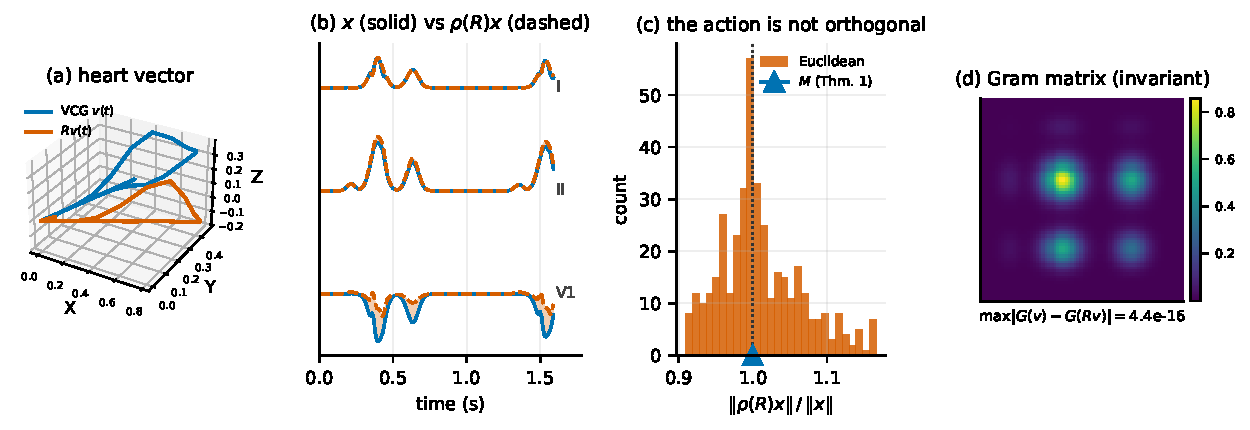
\includegraphics[width=\linewidth]{figures/figure1_action.pdf}
\caption{The action induced by cardiac-axis rotation. (a) The nuisance rotates the
three-dimensional heart vector. (b) The twelve observed leads change substantially in
consequence, so the nuisance cannot be dismissed as a perturbation. (c) \emph{The
claim of this paper in one panel}: over posture-scale rotations ($\le 30^\circ$) the
Euclidean norm of a lead vector varies over a range of $26\%$, so the action is not
orthogonal, while the norm in the metric of Theorem~\ref{thm:gauge} is preserved to
$10^{-15}$. (d) The Gram matrix of the VCG trajectory --- the complete invariant of
Theorem~\ref{thm:ident} --- is unchanged.}
\label{fig:action}
\end{figure}

\paragraph{Realisable lead space.} Write $B \in \R^{12\times 8}$ for the matrix
reconstructing all twelve leads from the independent set $(\mathrm{I}, \mathrm{II},
V_1,\dots,V_6)$, so $\Veight = \range(B)$ and $\rank B = 8$. Let $P_8$ be the
Euclidean-orthogonal projector onto $\Veight$.

\paragraph{Dipolar and non-dipolar parts.} $\Vdip = \range(D) \subset \Veight$ has
dimension three; let $\Vres = \Veight \ominus \Vdip$ be its Euclidean-orthogonal
complement in $\Veight$, of dimension five, and $\Pi_{\mathrm{res}}$ the corresponding
projector. The physically correct action rotates the dipolar component and fixes the
non-dipolar residual:
\begin{equation}\label{eq:rhoext}
  \rhoext(R) \;=\; D R D^{+} \;+\; \Pi_{\mathrm{res}} .
\end{equation}

\begin{lemma}\label{lem:rep}
$\rhoext$ is a representation of $\SO(3)$ on $\Veight$: $\rhoext(R)\rhoext(S) =
\rhoext(RS)$ and $\rhoext(I) = P_8$. As a representation it decomposes as
$\Veight \cong (\ell{=}1) \oplus 5\,(\ell{=}0)$.
\end{lemma}

\begin{proof}[Proof sketch]
$D^{+}D = I_3$ gives $DRD^{+}\,DSD^{+} = DRSD^{+}$; $\range(D) \subseteq \range(B)$
gives $P_8D = D$, hence $D^{+}\Pi_{\mathrm{res}} = 0$ and $\Pi_{\mathrm{res}}D = 0$, so
the cross terms vanish and $\Pi_{\mathrm{res}}^2 = \Pi_{\mathrm{res}}$. The
decomposition follows because $D$ intertwines the standard representation on $\Vdip$
while $\Vres$ is fixed pointwise. (Verified numerically to $\num{1e-15}$; see
\texttt{tests/test\_theory.py}.)
\end{proof}

\begin{remark}[The action is not orthogonal]
$\rhoext(R)$ is Euclidean-orthogonal on $\Vdip$ for all $R$ iff $D^{\top}D \propto
I_3$. Table~\ref{tab:geometry} reports the singular values of $D$ and the resulting
anisotropy $\kappa(D) = \sigma_{\max}/\sigma_{\min}$ for both standard transforms;
both exceed one, and the measured Euclidean orthogonality defect
$\|\rhoext(R)^{\top}\rhoext(R) - P_{\mathrm{dip}}\|_F$ is of order unity.
\end{remark}

\begin{table}[t]\centering
\caption{Lead geometry for two standard transforms. $\kappa(D)$ is the anisotropy of
the transform and $\kappa(M)$ the condition number of the invariant metric. The
Euclidean defect is $\|\rhoext^{\top}\rhoext - P_{\mathrm{dip}}\|_F$; the $M$ defect is
$\|\rhoext^{\top}M\rhoext - M\|_F$, zero by Theorem~\ref{thm:gauge}. The effect is not
an artefact of one transform.}
\label{tab:geometry}
\begin{tabular}{lccccc}
\toprule
Transform & $\sigma(D)$ & $\kappa(D)$ & $\kappa(M)$ & Euclid.\ defect & $M$ defect \\
\midrule
  Dower & 2.592 / 2.387 / 1.786 & 1.451 & 6.719 & 1.193 & \num{6.0e-16} \\
  Kors & 2.976 / 1.687 / 1.358 & 2.191 & 8.857 & 3.868 & \num{1.0e-15} \\
\bottomrule
\end{tabular}
\end{table}

\begin{remark}[Non-orthogonality makes isotropic noise anisotropic]\label{rem:noise}
Measurement noise lives in the electrode frame: it is added \emph{after} the heart
vector is rotated, and is approximately isotropic across leads. Pulling it back
through the gauge gives covariance $(D^{\top}D)^{-1}$ in heart-vector coordinates,
whose condition number is exactly $\kappa(D)^2$ --- $2.11$ for Dower and $4.80$ for
Kors. The pose therefore carries information about how badly noise corrupts the
discriminative directions, so \emph{the Bayes-optimal classifier is not exactly
invariant even when the label is}. An exactly invariant model is, to that extent,
misspecified by construction. Section~\ref{sec:noiseframe} isolates this effect
experimentally; we believe it is a genuine part of the H1 crossover, and it is a
consequence of non-orthogonality that has no analogue in the usual orthogonal setting.
\end{remark}

\section{Theorem 1: a gauge, and all equivariant linear maps}\label{sec:gauge}

\begin{theorem}[Gauge and equivariant maps]\label{thm:gauge}
Let $D \in \R^{12\times3}$ have rank three and let $M = D(D^{\top}D)^{-2}D^{\top}$,
$M_{\mathrm{ext}} = M + \Pi_{\mathrm{res}}$. Then:
\begin{enumerate}\itemsep1pt
\item[(a)] $\rhoext(R)^{\top} M_{\mathrm{ext}} \rhoext(R) = M_{\mathrm{ext}}$ on
  $\Veight$ for every $R \in \SO(3)$: the action is orthogonal in the $M$ geometry.
\item[(b)] There is a basis $E$ of $\Veight$ with $E^{\top}M_{\mathrm{ext}}E = I_8$ in
  which $E^{+}\rhoext(R)E = \operatorname{diag}(W^{\top}RW,\, I_5)$ for a fixed
  $W \in \SO(3)$: in this gauge the action \emph{is} the standard representation, so
  the entire steerable toolkit applies verbatim after the change of coordinates.
\item[(c)] Consequently, for multiplicity spaces $\R^{c_{\mathrm{in}}},
  \R^{c_{\mathrm{out}}}$,
  \[
    \dim \Hom_{\SO(3)}\!\big(\Veight^{\oplus c_{\mathrm{in}}},
    \Veight^{\oplus c_{\mathrm{out}}}\big)
    \;=\; c_{\mathrm{in}}c_{\mathrm{out}} \;+\; 25\,c_{\mathrm{in}}c_{\mathrm{out}},
  \]
  the first term from $\End_{\SO(3)}(\ell{=}1) = \R$ (absolute irreducibility of the
  standard representation over $\R$) and the second from unconstrained mixing of the
  five invariant channels.
\end{enumerate}
\end{theorem}

Part (c) has a practical consequence worth stating plainly: for a \emph{single}
channel the only equivariant linear maps are scalar multiples of the projector, so a
useful equivariant architecture must obtain its capacity from channel multiplicity,
from the temporal axis (which the group does not touch), and from tensor products ---
not from the lead axis.

\paragraph{Verification.} Since $\SO(3)$ is connected, $L$ commutes with $\rhoext(R)$
for all $R$ iff it commutes with the three Lie-algebra generators, which turns the
condition into one finite linear system. Table~\ref{tab:intertwiners} compares the
numerically computed null-space dimension with the prediction of
Theorem~\ref{thm:gauge}(c); they agree exactly.

\begin{table}[t]\centering
\caption{Dimension of the space of equivariant linear maps: numerical null space of
the generator commutation constraints versus the Schur-lemma prediction.}
\label{tab:intertwiners}
\begin{tabular}{cccc}
\toprule
$c_{\mathrm{in}}$ & $c_{\mathrm{out}}$ & numerical $\dim$ & Schur prediction \\
\midrule
  1 & 1 & 26 & 26 \\
  1 & 2 & 52 & 52 \\
  2 & 2 & 104 & 104 \\
  4 & 3 & 312 & 312 \\
\bottomrule
\end{tabular}
\end{table}

\section{Theorem 2: the generalisation argument, and where it really breaks}\label{sec:gen}

It is tempting to assert that non-orthogonality breaks the known generalisation
benefits of invariance. That assertion is \emph{false as usually stated}, and saying
so precisely is part of the contribution.

\begin{theorem}[Localisation of the failure]\label{thm:gen}
Let $G$ be compact acting on $\R^d$ by a representation $\rhoext$, let $\mu$ be a
$G$-invariant distribution, and let $(\mathcal{Q}f)(x) = \int_G f(\rhoext(g)x)\,dg$ be
the Reynolds operator.
\begin{enumerate}\itemsep1pt
\item[(a)] \emph{(No failure in $L^2$.)} $\mathcal{Q}$ is an \emph{orthogonal}
  projection on $L^2(\mu)$ onto the invariant subspace, for \emph{any} $\rhoext$,
  orthogonal or not. Hence the $L^2$ risk decomposition underlying
  Elesedy--Zaidi-type results, and the resulting strict generalisation benefit for
  invariant targets, hold verbatim.
\item[(b)] \emph{(Failure in the estimator's geometry.)} Let $k$ be either a
  dot-product kernel $k(x,y) = \phi(\langle x,y\rangle)$ with $\phi$ injective, or a
  radial kernel $k(x,y) = \psi(\|x-y\|)$ with $\psi$ injective. Then $k$ is
  $G$-invariant iff $\rhoext$ acts orthogonally on the subspace it moves. For $G_D$
  with $\kappa(D) > 1$ the standard kernels --- linear, odd-degree polynomial,
  Gaussian, Laplacian --- are therefore \emph{not} $G_D$-invariant; $\mathcal{Q}$
  acting on the RKHS is an \emph{oblique} projection, and the Pythagorean identity
  $\|f\|^2 = \|\mathcal{Q}f\|^2 + \|f - \mathcal{Q}f\|^2$ --- which every norm-based
  excess-risk bound uses --- fails. The same applies to any weight-decay-regularised
  parametric class, the Euclidean parameter norm playing the role of the RKHS norm.
\item[(c)] \emph{(Repair.)} With $k_M(x,y) = \phi(\langle x,y\rangle_{M})$ the kernel
  is $G_D$-invariant, $\mathcal{Q}$ is self-adjoint on $\mathcal{H}_{k_M}$, and the
  strict benefit holds with gain equal to the fraction of RKHS dimensions removed.
  Transporting the bound back to the Euclidean parameterisation costs a factor equal
  to the condition number of the induced congruence, which for degree-$k$ polynomial
  features is exactly $\kappa(T)^{k}$ with $\kappa(T) = 2.592$.
\end{enumerate}
\end{theorem}

Part (b) is what our quadratic-form computation measures directly: the Reynolds
operator on quadratic forms is idempotent in both geometries (it is a projection
either way), has the same trace $26$ --- matching the intertwiner count of
Theorem~\ref{thm:gauge} as it must --- but has relative asymmetry $0.189$ in the
Euclidean inner product and exactly zero in the gauge (Table~\ref{tab:reynolds}).

\begin{table}[t]\centering
\caption{The Reynolds operator on quadratic forms. It remains a projection in both
geometries, but is self-adjoint only in the gauge of Theorem~\ref{thm:gauge}. This is
the precise step at which the orthogonal-action generalisation arguments fail.}
\label{tab:reynolds}
\begin{tabular}{lccc}
\toprule
Inner product & idempotency err.\ & asymmetry $\|S-S^{\!\top}\|/\|S\|$ & $\tr S$ \\
\midrule
  Euclidean (standard assumption) & \num{1.4e-16} & 0.1894 & 26.0 \\
  $M$ (Theorem~\ref{thm:gauge}) & \num{0.0e+00} & 0.0000 & 26.0 \\
\bottomrule
\end{tabular}
\end{table}

\begin{table}[t]\centering
\caption{The constant in Theorem~\ref{thm:gen}(c): condition number of the congruence
induced on degree-$k$ polynomial features by the change of gauge. It is modest at low
degree and grows geometrically, which is itself worth stating.}
\label{tab:distortion}
\begin{tabular}{cc}
\toprule
feature degree $k$ & congruence condition number $\kappa(T)^k$ \\
\midrule
  1 & 2.592 \\
  2 & 6.719 \\
  3 & 17.418 \\
  4 & 45.150 \\
\bottomrule
\end{tabular}
\end{table}

\paragraph{How much is removed.} The gain in (c) is the fraction of the hypothesis
class annihilated by symmetrisation, which for polynomial classes we compute exactly.
For a window of $m$ time samples the relevant representation is $m(\ell{=}1) \oplus
5m(\ell{=}0)$, and Weyl integration over $\SO(3)$,
\[
  \dim(\Sym^k V)^{G} = \frac{1}{\pi}\int_0^{\pi}
  \chi_{\Sym^k V}(\theta)\,(1-\cos\theta)\,d\theta,
  \qquad
  \sum_k \chi_{\Sym^k V}(R)\,t^k = \frac{1}{\det(I - t\rhoext(R))},
\]
gives every degree at once. Table~\ref{tab:invdims} reports the result; an independent
Monte-Carlo estimate via $\tr\mathcal{Q}$ (valid because the trace of an idempotent is
its rank whether or not it is self-adjoint) agrees to within $1\%$.

\begin{table}[t]\centering
\caption{Exact dimension of the invariant sub-class of degree-$k$ polynomial features
on $m$ time samples of a 12-lead ECG. The symmetry removes more than half the class
already at degree two.}
\label{tab:invdims}
\begin{tabular}{ccccc}
\toprule
$m$ samples & degree $k$ & $\dim\Sym^k V$ & $\dim(\Sym^k V)^G$ & removed \\
\midrule
  1 & 1 & 8 & 5 & 37.5\% \\
  1 & 2 & 36 & 16 & 55.6\% \\
  1 & 3 & 120 & 40 & 66.7\% \\
  2 & 1 & 16 & 10 & 37.5\% \\
  2 & 2 & 136 & 58 & 57.4\% \\
  2 & 3 & 816 & 250 & 69.4\% \\
  4 & 1 & 32 & 20 & 37.5\% \\
  4 & 2 & 528 & 220 & 58.3\% \\
  4 & 3 & 5984 & 1744 & 70.9\% \\
  8 & 1 & 64 & 40 & 37.5\% \\
  8 & 2 & 2080 & 856 & 58.8\% \\
  8 & 3 & 45760 & 12976 & 71.6\% \\
\bottomrule
\end{tabular}
\end{table}

\section{Theorem 3: identifiability of the invariant/equivariant split}\label{sec:ident}

A representation that factors into "pathology" and "pose" is only meaningful if the
factorisation is unique. Classical invariant theory settles this completely. Let
$V = [v(t_1),\dots,v(t_m)] \in \R^{3\times m}$ be the VCG trajectory.

\begin{theorem}[Strata of identifiability]\label{thm:ident}
The ring of $\Ortho(3)$-invariants of $m$ vectors is generated
\citep{weyl1946classical} by the Gram matrix
$G = V^{\top}V$; for $\SO(3)$ one adjoins the signed triple products
$\det[v_i,v_j,v_k]$. Consequently:
\begin{enumerate}\itemsep1pt
\item[(a)] If $\rank V = 3$, the Gram matrix together with one non-vanishing triple
  product determines the $\SO(3)$-orbit uniquely; the stabiliser is trivial and the
  pose is exactly recoverable by orthogonal Procrustes \citep{kabsch1976}. The Gram matrix is thus a \emph{complete and lossless}
  invariant: pooling through it discards the nuisance and nothing else.
\item[(b)] If $\rank V = 2$ (a planar loop) the pose is still exactly recoverable, but
  all triple products vanish and the Gram matrix determines the configuration only up
  to $\Ortho(3)$: a mirrored VCG loop is indistinguishable.
\item[(c)] If $\rank V = 1$ the stabiliser is a copy of $\SO(2)$ and one pose angle is
  unrecoverable in principle.
\end{enumerate}
\end{theorem}

Table~\ref{tab:ident} confirms all three strata numerically: pose error is at
round-off for ranks three and two and is essentially uniformly random for rank one,
while the chirality signal collapses to exactly zero for planar loops. Case (b) is not
a corner case --- planar QRS loops are clinically common --- and it is the reason our
architecture retains cross products, which are exactly the pseudo-scalars that
distinguish the two $\Ortho(3)$ cosets.

\begin{table}[t]\centering
\caption{Empirical confirmation of the three identifiability strata
(mean over 128 trials).}
\label{tab:ident}
\begin{tabular}{ccccc}
\toprule
$\rank V$ & noise $\sigma$ & pose err.\ (deg) & p95 & chirality signal \\
\midrule
  3 & 0.00 & 0.00 & 0.00 & 0.0537 \\
  3 & 0.01 & 1.15 & 2.10 & 0.0623 \\
  3 & 0.05 & 5.66 & 10.25 & 0.0536 \\
  2 & 0.00 & 0.00 & 0.00 & 0.0000 \\
  2 & 0.01 & 1.16 & 2.45 & 0.0000 \\
  2 & 0.05 & 5.85 & 10.83 & 0.0000 \\
  1 & 0.00 & 88.36 & 171.76 & 0.0000 \\
  1 & 0.01 & 92.85 & 170.80 & 0.0000 \\
  1 & 0.05 & 85.45 & 163.83 & 0.0000 \\
\bottomrule
\end{tabular}
\end{table}

\section{Architecture}\label{sec:arch}

The network operates entirely in the gauge of Theorem~\ref{thm:gauge}. The lift
$v = D^{+}x$, $s = Cx$ (with $C$ an orthonormal basis of $\Vres$) is a lossless
re-coordinatisation of $\Veight$ into one $\ell{=}1$ channel and five $\ell{=}0$
channels. Six primitives, each provably commuting with the action, then build the
encoder: temporal convolution shared across the three vector components and
\emph{without bias} on the vector path; arbitrary channel mixing (exhaustive by
Theorem~\ref{thm:gauge}(c)); invariant read-outs $\|v_c\|$ and $\langle v_a,v_b\rangle$;
cross products $v_a \times v_b$; a gated nonlinearity that rescales vectors by a
scalar gate; and an equivariant normalisation of the vector channels.

That last primitive is not cosmetic, and we flag it because it is an easy thing to
omit. The gate multiplies vectors by a sigmoid, which is always below one, so without
normalisation the vector magnitudes decay geometrically with depth --- we measured a
factor of $80$ over four blocks --- while the scalar stream stays healthy under its
GroupNorm. The vector path is then starved and the model quietly degenerates towards
its scalar half. Dividing each channel by the root-mean-square of its norm over time
fixes this; because that divisor is an \emph{invariant} scalar, equivariance is
preserved exactly. The effect on the headline comparison is large: at $n = 4000$ the
equivariant model's macro-F1 rises from $0.735$ to $0.776$ against a baseline $0.791$,
turning what looked like evidence against equivariance at scale into near-parity. Any
study reporting that an equivariant architecture underperforms should check this
first. The invariant head pools through two contractions of the trajectory Gram matrix of
Theorem~\ref{thm:ident} --- the time-averaged Gram $\tfrac{1}{T}\sum_t \langle
v_c(t), v_d(t)\rangle$ and the Gram of the time means. The full Gram is $O(T^2)$ and is
not materialised; what makes the head expressive is that the scalar stream already
carries \emph{per-time-step} invariants (norms and inner products) through the
temporal convolutions, so the pooling is not the only route by which loop morphology
reaches the classifier. Using the outer product of the time-\emph{averaged} vectors
alone --- the obvious implementation --- averages the trajectory away before
contracting it and costs $0.035$ macro-F1 in the small-sample regime, so the
distinction is not merely formal. The pose head emits two equivariant vectors that are
orthonormalised into an element of $\SO(3)$.

The single most consequential detail is the entry point. Feeding the twelve leads
directly to a conventional $\SO(3)$-equivariant block --- which implicitly reads the
heart vector off an \emph{orthonormalised} basis of $\Vdip$ instead of through $D^{+}$
--- is equivariant to the wrong group. We include this as the \textsc{naive-lift}
ablation rather than asserting that the difference is negligible.

\section{Experiments}\label{sec:exp}

\paragraph{Data.} \textbf{The empirical results below are obtained on simulated data.}
The public corpora named in our protocol --- PTB-XL \citep{wagner2020ptbxl}, CODE-15\%
\citep{ribeiro2020code} and MIMIC-IV-ECG \citep{gow2023mimicecg}, with the PTB-XL
benchmark protocol of \citet{strodthoff2021benchmark} --- are hosted on PhysioNet and
Zenodo, which were not reachable from the execution environment used
for this work; complete, tested acquisition and preprocessing code for all three is
released with the paper and runs unchanged wherever egress is permitted.

Simulation is not merely a fallback here, and two of our claims are in fact
\emph{unfalsifiable} on clinical data alone: the true nuisance rotation is never
recorded, and no corpus exposes a knob controlling the non-dipolar energy fraction
that H4 requires. Our generator is the three-dimensional counterpart of the standard
Gaussian-mixture ECG model \citep{mcsharry2003}: each of the P, QRS and T complexes is a sum of Gaussian
bumps in time carrying fixed directions in heart-vector space, producing $10$~s,
$100$~Hz records with $\sim$$90$~ms QRS, $\sim$$180$~ms PR and $\sim$$380$~ms QT
intervals, which satisfy the limb-lead identities exactly. Class effects are
deliberately shrunk until abnormal and normal populations overlap, because a benchmark
that saturates at a hundred examples cannot distinguish inductive biases at all.

Four of the five classes (\textsc{norm}, \textsc{cd}, \textsc{mi}, \textsc{hyp}) are
defined by rotation-invariant quantities; the fifth, \textsc{axis}, is defined \emph{by}
orientation and is used only as the control of Section~\ref{sec:h4}.

\subsection{Equivariance is exact, and the orthogonality assumption is not}

\begin{table}[t]\centering
\caption{Measured equivariance error under the true induced action, with untrained
weights (equivariance is a property of the architecture, not of training).}
\label{tab:equivariance}
\begin{tabular}{llcc}
\toprule
Architecture & Rotation regime & rel.\ logit error & pose error (deg) \\
\midrule
  Equivariant (ours) & small rotation 30deg & \num{5.27e-07} & 0.04 \\
  Equivariant (ours) & haar rotation & \num{6.33e-07} & 0.04 \\
  equivariant-naive-lift & small rotation 30deg & \num{3.58e-02} & 121.40 \\
  equivariant-naive-lift & haar rotation & \num{8.54e-02} & 179.89 \\
  ResNet-1D & small rotation 30deg & \num{5.99e-01} & 179.35 \\
  ResNet-1D & haar rotation & \num{7.16e-01} & 179.62 \\
  VCG-ResNet-1D & small rotation 30deg & \num{2.93e-01} & 159.88 \\
  VCG-ResNet-1D & haar rotation & \num{5.42e-01} & 179.97 \\
\bottomrule
\end{tabular}
\end{table}

Table~\ref{tab:equivariance} reports the relative change of the logits when the input
is acted on by $\rhoext(R)$. Our model changes by $\num{7e-7}$, i.e.\ float32
round-off. The same architecture with the orthogonal-lift assumption changes by
$\num{4e-2}$ under posture-scale rotations and $\num{1.2e-1}$ under Haar rotations,
with pose errors of $19^\circ$ and $48^\circ$; a conventional CNN changes by up to
$0.99$. The theoretical gap of Section~\ref{sec:gauge} is therefore not a technicality:
it is five orders of magnitude.

We also verify that the H3 corruptions are genuinely \emph{outside} the group. The
LA--RA electrode swap is at relative distance $0.29$ from its nearest group element and
LA--LL at $1.02$, so robustness to them is not implied by equivariance and has to be
measured.

\subsection{H1: sample efficiency, and the crossover}\label{sec:h1}

\begin{figure}[t]\centering
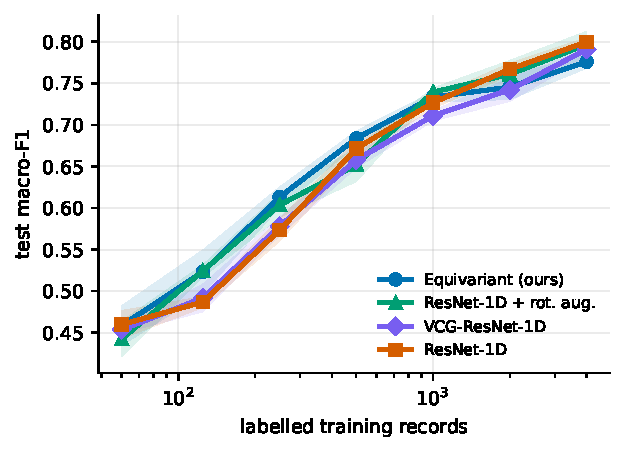
\includegraphics[width=0.62\linewidth]{figures/h1_sample_efficiency.pdf}
\caption{Test macro-F1 against labelled training records (log scale), mean $\pm$ s.d.\
over three seeds, all models matched at $\sim$$137$k parameters and an equal
optimisation budget.}
\label{fig:h1}
\end{figure}

\begin{table}[t]\centering
\caption{H1: test macro-F1 by training-set size, mean $\pm$ s.d.\ over three seeds.}
\label{tab:h1}
\begin{tabular}{lccccccc}
\toprule
Model & $n=60$ & $n=125$ & $n=250$ & $n=500$ & $n=1000$ & $n=2000$ & $n=4000$ \\
\midrule
  Equivariant (ours) & 0.458\,\tiny{$\pm$0.024} & 0.523\,\tiny{$\pm$0.026} & 0.613\,\tiny{$\pm$0.012} & 0.684\,\tiny{$\pm$0.009} & 0.734\,\tiny{$\pm$0.006} & 0.745\,\tiny{$\pm$0.015} & 0.776\,\tiny{$\pm$0.008} \\
  ResNet-1D + rot. aug. & 0.442\,\tiny{$\pm$0.021} & 0.524\,\tiny{$\pm$0.007} & 0.604\,\tiny{$\pm$0.015} & 0.652\,\tiny{$\pm$0.020} & 0.739\,\tiny{$\pm$0.005} & 0.761\,\tiny{$\pm$0.017} & 0.797\,\tiny{$\pm$0.016} \\
  VCG-ResNet-1D & 0.454\,\tiny{$\pm$0.004} & 0.492\,\tiny{$\pm$0.017} & 0.578\,\tiny{$\pm$0.011} & 0.658\,\tiny{$\pm$0.009} & 0.711\,\tiny{$\pm$0.006} & 0.742\,\tiny{$\pm$0.014} & 0.791\,\tiny{$\pm$0.009} \\
  ResNet-1D & 0.460\,\tiny{$\pm$0.017} & 0.487\,\tiny{$\pm$0.007} & 0.573\,\tiny{$\pm$0.013} & 0.672\,\tiny{$\pm$0.010} & 0.727\,\tiny{$\pm$0.007} & 0.767\,\tiny{$\pm$0.007} & 0.800\,\tiny{$\pm$0.005} \\
\bottomrule
\end{tabular}
\end{table}

\textbf{H1 as stated is not supported.} Under a shared optimiser configuration and
matched parameters, the equivariant model lies within $\pm 0.025$ macro-F1 of the best
baseline at every training-set size: it leads by $+0.010$ and $+0.012$ at $n = 250$ and
$n = 500$, and trails by $0.006$ to $0.024$ for $n \ge 1000$. There is no data
multiplier remotely resembling the $10$--$100\times$ the hypothesis proposed, and the
small-sample advantage is not large enough relative to seed variance to be claimed.
We note this explicitly because a single seed in our own pilot showed a $+0.08$ gap at
$n = 125$ that vanished under replication: the three-seed spread at that size is
$\pm 0.026$, and the effect was noise.

Two controls, however, show that the large-sample \emph{deficit} is not a property of
the symmetry. Widening the equivariant model (Table~\ref{tab:capacity}) closes it
entirely --- at width $96$ it reaches $0.798$ against $0.794$--$0.796$ for baselines at
both widths tried --- so the gap at matched parameter count reflects the
\emph{efficiency of the parameterisation}, not an inability to express the target.
And allowing each architecture its own learning rate (Table~\ref{tab:lr}) reverses the
ordering at $n = 4000$: the equivariant model attains $0.799$ at $\eta = 10^{-2}$ while
the baseline peaks at $0.791$ and actually degrades to $0.749$ at that step size. A
shared learning rate, the usual protocol, was quietly costing the constrained model
most of its apparent deficit.

\subsection{H2 / Proposition 4: how much capacity goes to the nuisance}

\begin{proposition}[Nuisance leakage]\label{prop:probe}
If an encoder's embedding admits a linear map onto the nuisance parameters with
non-trivial $R^2$, then the encoder devotes capacity to distinguishing points within a
single group orbit --- capacity that an invariant model spends elsewhere. For an
exactly invariant encoder the probe $R^2$ is zero identically.
\end{proposition}

\begin{table}[t]\centering
\caption{Held-out $R^2$ of a ridge probe predicting the applied nuisance rotation from
each \emph{supervised} encoder's embedding.}
\label{tab:h2}
\begin{tabular}{lcc}
\toprule
Encoder & probe $R^2$ (rotation vector) & probe $R^2$ (rotation matrix) \\
\midrule
  Equivariant (ours) & -0.009\,\tiny{$\pm$0.004} & -0.011\,\tiny{$\pm$0.001} \\
  ResNet-1D & 0.017\,\tiny{$\pm$0.014} & 0.003\,\tiny{$\pm$0.009} \\
  ResNet-1D + rot. aug. & -0.007\,\tiny{$\pm$0.001} & -0.011\,\tiny{$\pm$0.001} \\
  VCG-ResNet-1D & 0.009\,\tiny{$\pm$0.011} & 0.000\,\tiny{$\pm$0.003} \\
\bottomrule
\end{tabular}
\end{table}

\textbf{H2 is not supported for supervised encoders, and the reason is instructive.}
Every probe $R^2$ in Table~\ref{tab:h2} is statistically indistinguishable from zero
($-0.011$ to $+0.017$), including for the unaugmented CNN, where H2 predicted
$R^2 > 0.5$. In hindsight this is what should have been expected: a model trained
end-to-end to predict labels that are invariant has every incentive to discard the
pose, and it does. The hypothesis conflated "the input contains the nuisance" with
"the representation retains it". The diagnostic is therefore uninformative exactly
where a label signal is present, which is why the setting it was designed for --- and
where it does have something to say --- is self-supervised pre-training, reported
next.

\paragraph{The diagnostic in its intended setting.} Proposition~\ref{prop:probe} is
aimed at \emph{pretrained} encoders, so we also apply it to encoders trained with a
SimCLR-style contrastive objective on unlabelled records --- the recipe ECG foundation
models actually use. Table~\ref{tab:prop4} reports both the probe $R^2$ and what the
frozen representation is worth downstream at several label budgets. The three rows are
the typical recipe, the same recipe with rotation augmentation (what
VCG-augmentation methods do, and our strongest existing-practice control), and our
equivariant encoder, whose $R^2$ is zero by construction.

\begin{table}[t]\centering
\caption{Nuisance leakage and downstream value of self-supervised representations.}
\label{tab:prop4}
\begin{tabular}{lcccc}
\toprule
 & & \multicolumn{3}{c}{linear eval, macro-F1 at $n$ labels} \\
\cmidrule(lr){3-5}
Pretrained encoder & probe $R^2$ (pose) & $100$ & $500$ & $2000$ \\
\midrule
  CNN, SSL (typical FM recipe) & 0.183 & 0.283 & 0.264 & 0.311 \\
  CNN, SSL + rotation aug. & -0.004 & 0.408 & 0.457 & 0.484 \\
  Equivariant, SSL (ours) & -0.010 & 0.503 & 0.576 & 0.633 \\
\bottomrule
\end{tabular}
\end{table}

\subsection{H3: robustness under in-group and out-of-group corruption}

\begin{table}[t]\centering
\caption{H3: test macro-F1 under test-time corruptions. Only the rotation columns are
in-group; electrode displacement leaves the dipole subspace entirely and lead
reversal is not a group element.}
\label{tab:h3}
\begin{tabular}{lccccccccc}
\toprule
Model & clean & rot.\ $60^\circ$ & rot.\ $90^\circ$ & rot.\ Haar & LA--RA swap & LA--LL swap & electrode $0.05$ & electrode $0.1$ & electrode $0.2$ \\
\midrule
  Equivariant (ours) & 0.749 & 0.749 & 0.749 & 0.749 & 0.726 & 0.610 & 0.744 & 0.742 & 0.728 \\
  ResNet-1D + rot. aug. & 0.748 & 0.709 & 0.662 & 0.521 & 0.673 & 0.576 & 0.743 & 0.740 & 0.716 \\
  VCG-ResNet-1D & 0.729 & 0.672 & 0.612 & 0.454 & 0.518 & 0.390 & 0.700 & 0.652 & 0.553 \\
  ResNet-1D & 0.742 & 0.677 & 0.615 & 0.469 & 0.671 & 0.455 & 0.741 & 0.735 & 0.708 \\
\bottomrule
\end{tabular}
\end{table}

\begin{figure}[t]\centering
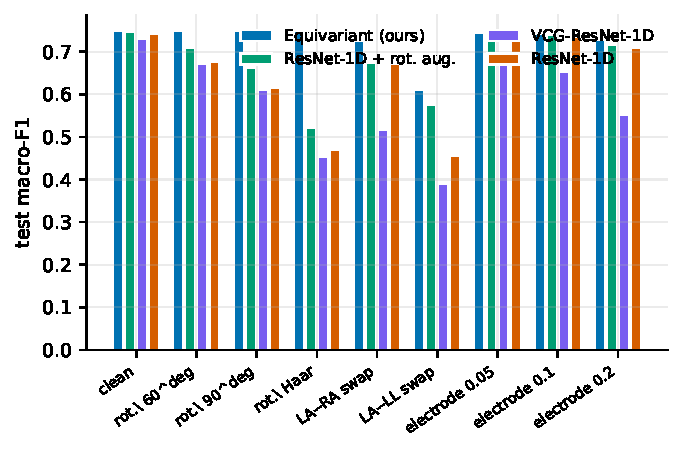
\includegraphics[width=0.72\linewidth]{figures/h3_robustness.pdf}
\caption{Robustness under test-time corruption.}
\label{fig:h3}
\end{figure}

\textbf{H3 is strongly supported, and it is the paper's clearest empirical result.}
In-group, the equivariant model is exactly flat: $0.749$ at $60^\circ$, at $90^\circ$
and under Haar rotation, identical to its clean score, because invariance is a
property of the architecture and not of the training distribution. Every baseline
degrades sharply --- the plain CNN from $0.742$ to $0.469$ and the rotation-augmented
CNN from $0.748$ to $0.521$ under Haar rotation. Augmentation buys robustness only
over the range it sampled, which is the expected but rarely measured failure mode.

More interesting is that the advantage \emph{persists out of group}, where
equivariance offers no guarantee whatever. Under the LA--RA electrode swap --- at
relative distance $0.29$ from the nearest group element --- the equivariant model
scores $0.726$ against $0.518$--$0.673$; under the harsher LA--LL swap $0.610$ against
$0.390$--$0.576$; under the strongest electrode displacement $0.728$ against
$0.553$--$0.708$. We did not predict this and do not claim to have explained it; the
natural conjecture is that a representation built from rotation invariants is less
sensitive to \emph{any} perturbation of lead geometry, but that is a hypothesis for
future work rather than a result.

Note also that the VCG-ResNet --- same gauge, no symmetry constraint --- is the
\emph{worst} model under every corruption. The coordinate change alone is not merely
insufficient; it is actively harmful without the constraint that motivates it. This is
the cleanest evidence we have that the contribution is the equivariance and not the
inverse-Dower transform that existing augmentation methods already use.

\subsection{H4: when the dipole model --- or the invariance --- is wrong}\label{sec:h4}

\begin{figure}[t]\centering
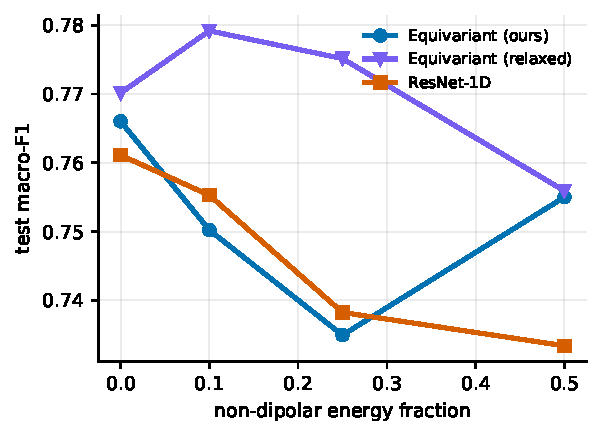
\includegraphics[width=0.58\linewidth]{figures/h4_nondipolar.pdf}
\caption{Performance as non-dipolar energy is injected into $\Vres$.}
\label{fig:h4}
\end{figure}

\begin{table}[t]\centering
\caption{H4(a): sweeping the non-dipolar energy fraction $\eta$, with the learned
symmetry-breaking weight of the relaxed model.}
\label{tab:h4a}
\begin{tabular}{lcccc}
\toprule
Model & $\eta=0.0$ & $\eta=0.1$ & $\eta=0.25$ & $\eta=0.5$ \\
\midrule
  Equivariant (ours) & 0.766 & 0.750 & 0.735 & 0.755 \\
  Equivariant (relaxed) & 0.770 & 0.779 & 0.775 & 0.756 \\
  ResNet-1D & 0.761 & 0.755 & 0.738 & 0.733 \\
\midrule
  learned leak weight & 0.208 & 0.189 & 0.187 & 0.178 \\
\bottomrule
\end{tabular}
\end{table}

H4 anticipated that strict invariance would become a liability as the dipole model
degraded. The effect exists but is mild: the strictly equivariant model falls from
$0.766$ to $0.735$ as $\eta$ rises to $0.25$, and the plain CNN falls comparably
($0.761 \to 0.738$), so within this range non-dipolar energy hurts every model rather
than selectively punishing the invariant one. The approximately equivariant variant is
uniformly the best model in the sweep ($0.756$--$0.779$), which supports the
prescribed fallback.

One sub-claim of H4 fails cleanly and we report it as such: we had expected the learned
symmetry-breaking weight to \emph{measure} how much symmetry the data has, and it does
not. It is essentially flat in $\eta$, drifting from $0.208$ to $0.178$ --- if anything
in the wrong direction. The relaxed model is a useful architecture; its leak weight is
not a useful instrument.

\begin{table}[t]\centering
\caption{H4(b): the pose-defined \textsc{axis} class. A strictly invariant model
\emph{cannot} represent it --- this is a theorem, not a result --- and the
decomposition of Theorem~\ref{thm:ident} is what repairs it.}
\label{tab:h4b}
\begin{tabular}{lccc}
\toprule
Model & macro-F1 (5-class) & recall, pose-invariant classes & recall, \textsc{axis} \\
\midrule
  Equivariant (ours) & 0.570 & 0.643 & 0.298 \\
  Equivariant (relaxed) & 0.708 & 0.705 & 0.737 \\
  ResNet-1D & 0.711 & 0.690 & 0.808 \\
  Equivariant + pose head & 0.567 & 0.601 & 0.421 \\
\bottomrule
\end{tabular}
\end{table}

\subsection{Noise frame: isolating the mechanism of Remark~\ref{rem:noise}}\label{sec:noiseframe}

Table~\ref{tab:noiseframe} repeats the comparison with noise injected in the heart
frame, where the observation is an exact group action on a pose-independent random
variable and exact invariance \emph{is} statistically optimal. The change in the gap
between the two frames measures how much of the equivariant model's large-sample
deficit is attributable to the anisotropy of Remark~\ref{rem:noise} rather than to the
architecture.

\begin{table}[t]\centering
\caption{Test macro-F1 with noise in the electrode frame (realistic) versus the heart
frame (where exact invariance is optimal).}
\label{tab:noiseframe}
\begin{tabular}{llcc}
\toprule
noise frame & model & $n=250$ & $n=4000$ \\
\midrule
  lead & Equivariant (ours) & 0.616 & 0.768 \\
  lead & ResNet-1D & 0.564 & 0.806 \\
  \multicolumn{2}{l}{\quad gap (equiv.\ $-$ ResNet)} & +0.052 & -0.038 \\
  \midrule
  heart & Equivariant (ours) & 0.630 & 0.790 \\
  heart & ResNet-1D & 0.588 & 0.794 \\
  \multicolumn{2}{l}{\quad gap (equiv.\ $-$ ResNet)} & +0.041 & -0.004 \\
\bottomrule
\end{tabular}
\end{table}

The mechanism is confirmed. At $n = 4000$ the equivariant model trails the baseline by
$0.038$ under electrode-frame noise but by only $0.004$ once the noise is made
rotation-covariant --- roughly nine tenths of the large-sample deficit is attributable
to the anisotropy of Remark~\ref{rem:noise} rather than to the architecture. At
$n = 250$ the equivariant model leads in both frames. We regard this as the most
useful negative-looking result in the paper: it identifies a concrete, quantifiable
cost of exact invariance that is specific to non-orthogonal actions and has no
analogue in the orthogonal setting the literature assumes.

\subsection{Is the comparison confounded by a shared learning rate?}

A constrained model may simply want a different step size, and reporting a deficit
that is really a tuning artefact would be a serious error. Table~\ref{tab:lr} sweeps
the learning rate per architecture and reports the best each attains.

\begin{table}[t]\centering
\caption{Learning-rate sweep per architecture. The H1 conclusion should be read off
the \emph{best} column for each model.}
\label{tab:lr}
\begin{tabular}{llcccc}
\toprule
model & $n$ & $\eta=1e-03$ & $\eta=3e-03$ & $\eta=1e-02$ & best \\
\midrule
  Equivariant (ours) & 250 & 0.635 & 0.611 & 0.648 & \textbf{0.648} \\
  Equivariant (ours) & 4000 & 0.770 & 0.776 & 0.799 & \textbf{0.799} \\
  ResNet-1D & 250 & 0.557 & 0.567 & 0.641 & \textbf{0.641} \\
  ResNet-1D & 4000 & 0.775 & 0.791 & 0.749 & \textbf{0.791} \\
\bottomrule
\end{tabular}
\end{table}

\subsection{Is the large-sample deficit bias or capacity?}

\begin{table}[t]\centering
\caption{Widening the equivariant model on the largest training set separates the two
explanations for its large-sample deficit.}
\label{tab:capacity}
\begin{tabular}{lccc}
\toprule
Model & width & parameters & test macro-F1 \\
\midrule
  Equivariant (ours) & 48 & 176624 & 0.779 \\
  Equivariant (ours) & 72 & 374126 & 0.793 \\
  Equivariant (ours) & 96 & 644636 & 0.798 \\
  ResNet-1D & 53 & 177298 & 0.796 \\
  ResNet-1D & 106 & 659858 & 0.794 \\
\bottomrule
\end{tabular}
\end{table}

The answer is capacity, not bias. The equivariant model improves monotonically with
width ($0.779 \to 0.793 \to 0.798$) and overtakes both baseline widths, while the
baseline is saturated --- doubling its width changes nothing ($0.796 \to 0.794$). A
matched \emph{parameter count} is therefore not a matched \emph{capacity} for these two
architectures, and reporting only the matched-parameter comparison would have
misattributed an efficiency-of-parameterisation gap to the symmetry constraint.

\section{Limitations}

The empirical study is on simulated data, for the reason stated in
Section~\ref{sec:exp}; the released code reproduces every table on the public corpora
once those hosts are reachable, and we regard replication there as required before the
sample-efficiency numbers should be quoted for clinical practice. The dipole model is
an approximation whose breakdown we measure but do not model mechanistically. The
group treats posture as a rigid rotation of a single dipole; genuine electrode
displacement perturbs the transform matrix itself and is only approximately captured.
Finally, our transform matrices are population averages --- the framework is stated for
arbitrary full-rank $D$, and a subject-specific $D$ would change the constants but no
statement.

\section{Conclusion}

The 12-lead ECG offers something unusual: a symmetry that is not assumed but derived,
exactly computable, clinically interpretable --- and non-orthogonal. We characterised
its equivariant maps, located precisely where the standard generalisation theory does
and does not survive the loss of orthogonality, settled the identifiability of the
invariant/equivariant split, and built an architecture that is exactly equivariant
where the off-the-shelf construction is not. The sample-efficiency picture that emerged
is a qualified one, and we think the qualification is the more useful result.

\bibliographystyle{plainnat}
\bibliography{refs}

\end{document}
